\documentclass[]{article}
\usepackage{lmodern}
\usepackage{amssymb,amsmath}
\usepackage{ifxetex,ifluatex}
\usepackage{fixltx2e} % provides \textsubscript
\ifnum 0\ifxetex 1\fi\ifluatex 1\fi=0 % if pdftex
  \usepackage[T1]{fontenc}
  \usepackage[utf8]{inputenc}
\else % if luatex or xelatex
  \ifxetex
    \usepackage{mathspec}
  \else
    \usepackage{fontspec}
  \fi
  \defaultfontfeatures{Ligatures=TeX,Scale=MatchLowercase}
\fi
% use upquote if available, for straight quotes in verbatim environments
\IfFileExists{upquote.sty}{\usepackage{upquote}}{}
% use microtype if available
\IfFileExists{microtype.sty}{%
\usepackage{microtype}
\UseMicrotypeSet[protrusion]{basicmath} % disable protrusion for tt fonts
}{}
\usepackage[margin=1in]{geometry}
\usepackage{hyperref}
\hypersetup{unicode=true,
            pdftitle={Reproducible Research Course Project 1},
            pdfauthor={Sheila Braun},
            pdfborder={0 0 0},
            breaklinks=true}
\urlstyle{same}  % don't use monospace font for urls
\usepackage{color}
\usepackage{fancyvrb}
\newcommand{\VerbBar}{|}
\newcommand{\VERB}{\Verb[commandchars=\\\{\}]}
\DefineVerbatimEnvironment{Highlighting}{Verbatim}{commandchars=\\\{\}}
% Add ',fontsize=\small' for more characters per line
\usepackage{framed}
\definecolor{shadecolor}{RGB}{248,248,248}
\newenvironment{Shaded}{\begin{snugshade}}{\end{snugshade}}
\newcommand{\KeywordTok}[1]{\textcolor[rgb]{0.13,0.29,0.53}{\textbf{#1}}}
\newcommand{\DataTypeTok}[1]{\textcolor[rgb]{0.13,0.29,0.53}{#1}}
\newcommand{\DecValTok}[1]{\textcolor[rgb]{0.00,0.00,0.81}{#1}}
\newcommand{\BaseNTok}[1]{\textcolor[rgb]{0.00,0.00,0.81}{#1}}
\newcommand{\FloatTok}[1]{\textcolor[rgb]{0.00,0.00,0.81}{#1}}
\newcommand{\ConstantTok}[1]{\textcolor[rgb]{0.00,0.00,0.00}{#1}}
\newcommand{\CharTok}[1]{\textcolor[rgb]{0.31,0.60,0.02}{#1}}
\newcommand{\SpecialCharTok}[1]{\textcolor[rgb]{0.00,0.00,0.00}{#1}}
\newcommand{\StringTok}[1]{\textcolor[rgb]{0.31,0.60,0.02}{#1}}
\newcommand{\VerbatimStringTok}[1]{\textcolor[rgb]{0.31,0.60,0.02}{#1}}
\newcommand{\SpecialStringTok}[1]{\textcolor[rgb]{0.31,0.60,0.02}{#1}}
\newcommand{\ImportTok}[1]{#1}
\newcommand{\CommentTok}[1]{\textcolor[rgb]{0.56,0.35,0.01}{\textit{#1}}}
\newcommand{\DocumentationTok}[1]{\textcolor[rgb]{0.56,0.35,0.01}{\textbf{\textit{#1}}}}
\newcommand{\AnnotationTok}[1]{\textcolor[rgb]{0.56,0.35,0.01}{\textbf{\textit{#1}}}}
\newcommand{\CommentVarTok}[1]{\textcolor[rgb]{0.56,0.35,0.01}{\textbf{\textit{#1}}}}
\newcommand{\OtherTok}[1]{\textcolor[rgb]{0.56,0.35,0.01}{#1}}
\newcommand{\FunctionTok}[1]{\textcolor[rgb]{0.00,0.00,0.00}{#1}}
\newcommand{\VariableTok}[1]{\textcolor[rgb]{0.00,0.00,0.00}{#1}}
\newcommand{\ControlFlowTok}[1]{\textcolor[rgb]{0.13,0.29,0.53}{\textbf{#1}}}
\newcommand{\OperatorTok}[1]{\textcolor[rgb]{0.81,0.36,0.00}{\textbf{#1}}}
\newcommand{\BuiltInTok}[1]{#1}
\newcommand{\ExtensionTok}[1]{#1}
\newcommand{\PreprocessorTok}[1]{\textcolor[rgb]{0.56,0.35,0.01}{\textit{#1}}}
\newcommand{\AttributeTok}[1]{\textcolor[rgb]{0.77,0.63,0.00}{#1}}
\newcommand{\RegionMarkerTok}[1]{#1}
\newcommand{\InformationTok}[1]{\textcolor[rgb]{0.56,0.35,0.01}{\textbf{\textit{#1}}}}
\newcommand{\WarningTok}[1]{\textcolor[rgb]{0.56,0.35,0.01}{\textbf{\textit{#1}}}}
\newcommand{\AlertTok}[1]{\textcolor[rgb]{0.94,0.16,0.16}{#1}}
\newcommand{\ErrorTok}[1]{\textcolor[rgb]{0.64,0.00,0.00}{\textbf{#1}}}
\newcommand{\NormalTok}[1]{#1}
\usepackage{graphicx,grffile}
\makeatletter
\def\maxwidth{\ifdim\Gin@nat@width>\linewidth\linewidth\else\Gin@nat@width\fi}
\def\maxheight{\ifdim\Gin@nat@height>\textheight\textheight\else\Gin@nat@height\fi}
\makeatother
% Scale images if necessary, so that they will not overflow the page
% margins by default, and it is still possible to overwrite the defaults
% using explicit options in \includegraphics[width, height, ...]{}
\setkeys{Gin}{width=\maxwidth,height=\maxheight,keepaspectratio}
\IfFileExists{parskip.sty}{%
\usepackage{parskip}
}{% else
\setlength{\parindent}{0pt}
\setlength{\parskip}{6pt plus 2pt minus 1pt}
}
\setlength{\emergencystretch}{3em}  % prevent overfull lines
\providecommand{\tightlist}{%
  \setlength{\itemsep}{0pt}\setlength{\parskip}{0pt}}
\setcounter{secnumdepth}{0}
% Redefines (sub)paragraphs to behave more like sections
\ifx\paragraph\undefined\else
\let\oldparagraph\paragraph
\renewcommand{\paragraph}[1]{\oldparagraph{#1}\mbox{}}
\fi
\ifx\subparagraph\undefined\else
\let\oldsubparagraph\subparagraph
\renewcommand{\subparagraph}[1]{\oldsubparagraph{#1}\mbox{}}
\fi

%%% Use protect on footnotes to avoid problems with footnotes in titles
\let\rmarkdownfootnote\footnote%
\def\footnote{\protect\rmarkdownfootnote}

%%% Change title format to be more compact
\usepackage{titling}

% Create subtitle command for use in maketitle
\newcommand{\subtitle}[1]{
  \posttitle{
    \begin{center}\large#1\end{center}
    }
}

\setlength{\droptitle}{-2em}
  \title{Reproducible Research Course Project 1}
  \pretitle{\vspace{\droptitle}\centering\huge}
  \posttitle{\par}
  \author{Sheila Braun}
  \preauthor{\centering\large\emph}
  \postauthor{\par}
  \predate{\centering\large\emph}
  \postdate{\par}
  \date{May 10, 2018}


\begin{document}
\maketitle

\subsubsection{Project Steps}\label{project-steps}

\paragraph{1. Read in the dataset.}\label{read-in-the-dataset.}

We load in required library, set some global options, and read in the
data to a dataframe called my usual default, ``df.'' Then we have a look
at the data set.

\begin{Shaded}
\begin{Highlighting}[]
\KeywordTok{options}\NormalTok{(}\DataTypeTok{digits =} \DecValTok{2}\NormalTok{, }\DataTypeTok{scipen =} \DecValTok{9999}\NormalTok{)}
\KeywordTok{library}\NormalTok{(chron)}
\end{Highlighting}
\end{Shaded}

\begin{verbatim}
## Warning: package 'chron' was built under R version 3.4.4
\end{verbatim}

\begin{Shaded}
\begin{Highlighting}[]
\KeywordTok{library}\NormalTok{(lattice)}
\NormalTok{df <-}\StringTok{ }\KeywordTok{read.csv}\NormalTok{(}\StringTok{"activity.csv"}\NormalTok{, }\DataTypeTok{head =} \OtherTok{TRUE}\NormalTok{)}
\KeywordTok{head}\NormalTok{(df, }\DecValTok{10}\NormalTok{)}
\end{Highlighting}
\end{Shaded}

\begin{verbatim}
##    steps       date interval
## 1     NA 2012-10-01        0
## 2     NA 2012-10-01        5
## 3     NA 2012-10-01       10
## 4     NA 2012-10-01       15
## 5     NA 2012-10-01       20
## 6     NA 2012-10-01       25
## 7     NA 2012-10-01       30
## 8     NA 2012-10-01       35
## 9     NA 2012-10-01       40
## 10    NA 2012-10-01       45
\end{verbatim}

\paragraph{2. Do a little data prep.}\label{do-a-little-data-prep.}

\begin{itemize}
\tightlist
\item
  Format the dates in the dataframe.
\end{itemize}

\begin{Shaded}
\begin{Highlighting}[]
\NormalTok{df}\OperatorTok{$}\NormalTok{date <-}\StringTok{ }\KeywordTok{strptime}\NormalTok{(df}\OperatorTok{$}\NormalTok{date, }\StringTok{"%Y-%m-%d"}\NormalTok{)}
\end{Highlighting}
\end{Shaded}

\begin{itemize}
\tightlist
\item
  Create a vector of dates.
\end{itemize}

\begin{Shaded}
\begin{Highlighting}[]
\NormalTok{dates <-}\StringTok{ }\NormalTok{df}\OperatorTok{$}\NormalTok{date}
\end{Highlighting}
\end{Shaded}

\begin{itemize}
\tightlist
\item
  Create a vector of unique dates.
\end{itemize}

\begin{Shaded}
\begin{Highlighting}[]
\NormalTok{uniqueDays <-}\StringTok{ }\KeywordTok{unique}\NormalTok{(df}\OperatorTok{$}\NormalTok{date)}
\end{Highlighting}
\end{Shaded}

\begin{itemize}
\tightlist
\item
  Create a vector of unique intervals.
\end{itemize}

\begin{Shaded}
\begin{Highlighting}[]
\NormalTok{uniqueInts <-}\StringTok{ }\KeywordTok{unique}\NormalTok{(df}\OperatorTok{$}\NormalTok{interval)}
\end{Highlighting}
\end{Shaded}

\begin{itemize}
\tightlist
\item
  Calculate the total number of unique dates.
\end{itemize}

\begin{Shaded}
\begin{Highlighting}[]
\NormalTok{totUniqueDays <-}\StringTok{ }\KeywordTok{length}\NormalTok{(uniqueDays)}
\end{Highlighting}
\end{Shaded}

\begin{itemize}
\tightlist
\item
  Calculate the total number of unique intervals.
\end{itemize}

\begin{Shaded}
\begin{Highlighting}[]
\NormalTok{totUniqueInts <-}\StringTok{ }\KeywordTok{length}\NormalTok{(uniqueInts)}
\end{Highlighting}
\end{Shaded}

\begin{itemize}
\tightlist
\item
  Create a list of unique days with their matching steps. That list
  contains what we need to calculate the total number of steps per day.
\end{itemize}

\begin{Shaded}
\begin{Highlighting}[]
\NormalTok{stepsDay <-}\StringTok{ }\KeywordTok{split}\NormalTok{(df}\OperatorTok{$}\NormalTok{steps, dates}\OperatorTok{$}\NormalTok{yday)}
\end{Highlighting}
\end{Shaded}

\begin{itemize}
\tightlist
\item
  Calculate the total number of steps per day.
\end{itemize}

\begin{Shaded}
\begin{Highlighting}[]
\NormalTok{totStepsDay <-}\StringTok{ }\KeywordTok{sapply}\NormalTok{(stepsDay, sum, }\DataTypeTok{na.rm=}\OtherTok{TRUE}\NormalTok{) }
\end{Highlighting}
\end{Shaded}

We have 61 unique days and 288 unique intervals.

\paragraph{3. Have a look at the day list, then create a histogram of
the total number of steps taken each
day.}\label{have-a-look-at-the-day-list-then-create-a-histogram-of-the-total-number-of-steps-taken-each-day.}

\begin{Shaded}
\begin{Highlighting}[]
\KeywordTok{str}\NormalTok{(totStepsDay)}
\end{Highlighting}
\end{Shaded}

\begin{verbatim}
##  Named int [1:61] 0 126 11352 12116 13294 15420 11015 0 12811 9900 ...
##  - attr(*, "names")= chr [1:61] "274" "275" "276" "277" ...
\end{verbatim}

\begin{Shaded}
\begin{Highlighting}[]
\KeywordTok{hist}\NormalTok{(totStepsDay, }\DataTypeTok{main =} \StringTok{"Histogram of Total Steps per Day"}\NormalTok{,}
     \DataTypeTok{xlab =} \StringTok{"Steps per Day"}\NormalTok{, }\DataTypeTok{ylab =} \StringTok{"Frequency"}\NormalTok{)}
\end{Highlighting}
\end{Shaded}

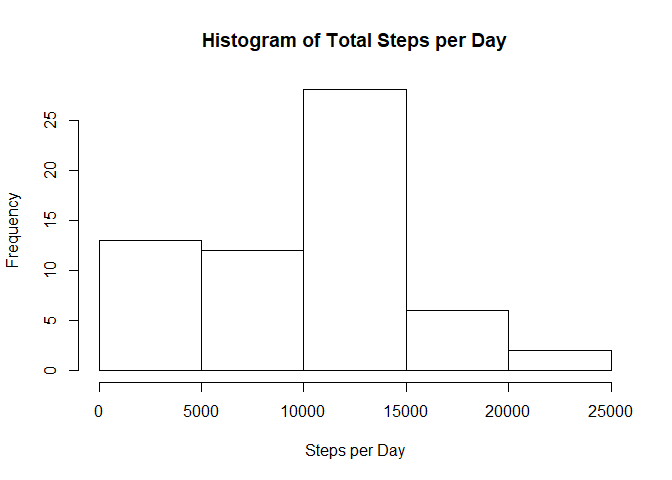
\includegraphics{Course_Project_1_for_Reproducible_Research_files/figure-latex/histsteps-1.pdf}

\begin{Shaded}
\begin{Highlighting}[]
\NormalTok{## And just to satisfly my need for tidiness, make "interval" into a separate factor variable. ##}

\NormalTok{df}\OperatorTok{$}\NormalTok{factInt <-}\StringTok{ }\KeywordTok{as.factor}\NormalTok{(df}\OperatorTok{$}\NormalTok{interval)}
\KeywordTok{head}\NormalTok{(df}\OperatorTok{$}\NormalTok{factInt)}
\end{Highlighting}
\end{Shaded}

\begin{verbatim}
## [1] 0  5  10 15 20 25
## 288 Levels: 0 5 10 15 20 25 30 35 40 45 50 55 100 105 110 115 120 ... 2355
\end{verbatim}

\paragraph{4. Next show the mean and median number of steps taken each
day.}\label{next-show-the-mean-and-median-number-of-steps-taken-each-day.}

\begin{Shaded}
\begin{Highlighting}[]
\NormalTok{mnsteps <-}\StringTok{ }\KeywordTok{mean}\NormalTok{(totStepsDay, }\DataTypeTok{na.rm =} \OtherTok{TRUE}\NormalTok{)}
\NormalTok{mdsteps <-}\StringTok{ }\KeywordTok{median}\NormalTok{(totStepsDay, }\DataTypeTok{na.rm =} \OtherTok{TRUE}\NormalTok{)}
\end{Highlighting}
\end{Shaded}

\begin{itemize}
\tightlist
\item
  Mean total steps is 9354.23.\\
\item
  Median total steps is 10395.
\end{itemize}

\paragraph{\texorpdfstring{5. What is the average daily activity
pattern? Make a time series plot (i.e.~type = ``l'') of the 5-minute
interval (x-axis) and the average number of steps taken, averaged across
all days
(y-axis)}{5. What is the average daily activity pattern? Make a time series plot (i.e.~type = l) of the 5-minute interval (x-axis) and the average number of steps taken, averaged across all days (y-axis)}}\label{what-is-the-average-daily-activity-pattern-make-a-time-series-plot-i.e.type-l-of-the-5-minute-interval-x-axis-and-the-average-number-of-steps-taken-averaged-across-all-days-y-axis}

\begin{Shaded}
\begin{Highlighting}[]
\NormalTok{intData <-}\StringTok{ }\KeywordTok{split}\NormalTok{(df}\OperatorTok{$}\NormalTok{steps, df}\OperatorTok{$}\NormalTok{interval)}
\NormalTok{avgStepsInt <-}\StringTok{ }\KeywordTok{sapply}\NormalTok{(intData, mean, }\DataTypeTok{na.rm =} \OtherTok{TRUE}\NormalTok{)}
\KeywordTok{plot}\NormalTok{(uniqueInts, avgStepsInt, }\DataTypeTok{type =} \StringTok{"l"}\NormalTok{,}
     \DataTypeTok{main =} \StringTok{"Time Series: Average Steps per Interval on a Given Day"}\NormalTok{,}
     \DataTypeTok{xlab =} \StringTok{"Interval"}\NormalTok{, }\DataTypeTok{ylab =} \StringTok{"Steps"}\NormalTok{)}
\end{Highlighting}
\end{Shaded}

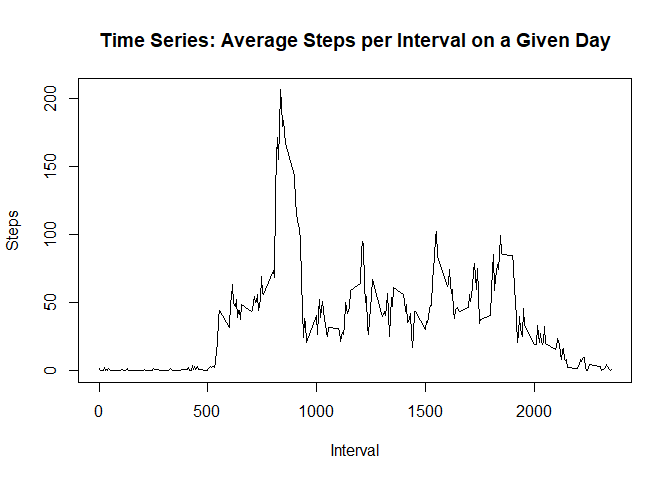
\includegraphics{Course_Project_1_for_Reproducible_Research_files/figure-latex/timeseries-1.pdf}

\begin{Shaded}
\begin{Highlighting}[]
\NormalTok{maxInt =}\StringTok{ }\KeywordTok{max}\NormalTok{(df}\OperatorTok{$}\NormalTok{interval)}
\end{Highlighting}
\end{Shaded}

People start out slow on most days and stay slow until about interval
500. Then they start moving around more, with rapidly increasing numbers
of steps until a very high peak of close to 200 steps per interval at
interval 835. After that peak, number of steps drops down to a range of
steps between about 25 and 100 that people seem to maintain until about
interval 1900, at which point activity decreases until it reaches 0 at
interval 2355.

\paragraph{6. Identify the 5-minute interval that, on average, contains
the maximum number of
steps}\label{identify-the-5-minute-interval-that-on-average-contains-the-maximum-number-of-steps}

\begin{Shaded}
\begin{Highlighting}[]
\NormalTok{maxIntDays <-}\StringTok{ }\KeywordTok{max}\NormalTok{(avgStepsInt, }\DataTypeTok{na.rm=}\OtherTok{TRUE}\NormalTok{)}
\NormalTok{maxIndex <-}\StringTok{ }\KeywordTok{as.numeric}\NormalTok{(}\KeywordTok{which}\NormalTok{(avgStepsInt }\OperatorTok{==}\StringTok{ }\NormalTok{maxIntDays))}
\NormalTok{maxInt <-}\StringTok{ }\NormalTok{uniqueInts[maxIndex]}
\KeywordTok{plot}\NormalTok{(uniqueInts, avgStepsInt, }\DataTypeTok{type =} \StringTok{"l"}\NormalTok{,}
     \DataTypeTok{main =} \StringTok{"Time Series: Maximum Steps per Interval on a Given Day"}\NormalTok{,}
     \DataTypeTok{xlab =} \StringTok{"Interval"}\NormalTok{, }\DataTypeTok{ylab =} \StringTok{"Steps"}\NormalTok{)}
\KeywordTok{abline}\NormalTok{(}\DataTypeTok{v=}\NormalTok{maxInt, }\DataTypeTok{col =} \StringTok{"red"}\NormalTok{, }\DataTypeTok{lwd =} \DecValTok{2}\NormalTok{)}
\end{Highlighting}
\end{Shaded}

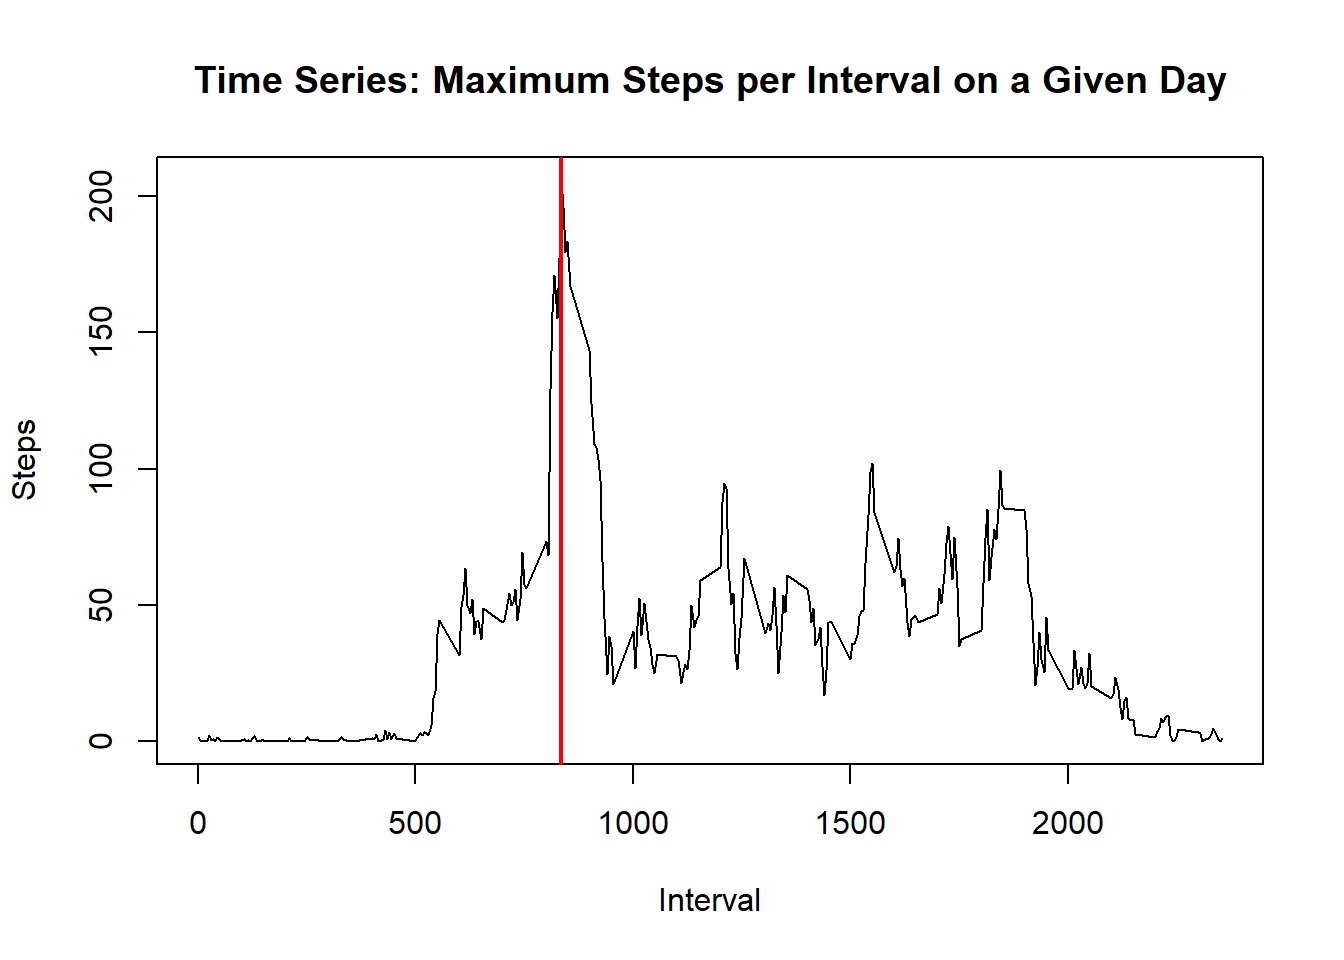
\includegraphics{Course_Project_1_for_Reproducible_Research_files/figure-latex/findMax-1.pdf}

The maximum average numbers of steps happens at interval 835 on a given
day.

\paragraph{7. Code to describe and show a strategy for imputing missing
data.}\label{code-to-describe-and-show-a-strategy-for-imputing-missing-data.}

The first question to answer is whether there is a pattern to the
missing data that might suggest an appropriate way to impute the missing
data. First, then, identify and pull out the missing cases and visualize
them to see if there is any kind of pattern.

\begin{Shaded}
\begin{Highlighting}[]
\NormalTok{missings <-}\StringTok{ }\NormalTok{df[}\OperatorTok{!}\KeywordTok{complete.cases}\NormalTok{(df}\OperatorTok{$}\NormalTok{steps),]}
\NormalTok{numMissing <-}\StringTok{ }\KeywordTok{sum}\NormalTok{(}\KeywordTok{is.na}\NormalTok{(df}\OperatorTok{$}\NormalTok{steps))}
\KeywordTok{str}\NormalTok{(missings)}
\end{Highlighting}
\end{Shaded}

\begin{verbatim}
## 'data.frame':    2304 obs. of  4 variables:
##  $ steps   : int  NA NA NA NA NA NA NA NA NA NA ...
##  $ date    : POSIXlt, format: "2012-10-01" "2012-10-01" ...
##  $ interval: int  0 5 10 15 20 25 30 35 40 45 ...
##  $ factInt : Factor w/ 288 levels "0","5","10","15",..: 1 2 3 4 5 6 7 8 9 10 ...
\end{verbatim}

\begin{Shaded}
\begin{Highlighting}[]
\KeywordTok{plot}\NormalTok{(missings}\OperatorTok{$}\NormalTok{date, missings}\OperatorTok{$}\NormalTok{interval, }\DataTypeTok{ylab =} \StringTok{"Interval Numbers"}\NormalTok{, }\DataTypeTok{xlab =} \StringTok{"Dates"}\NormalTok{)}
\end{Highlighting}
\end{Shaded}

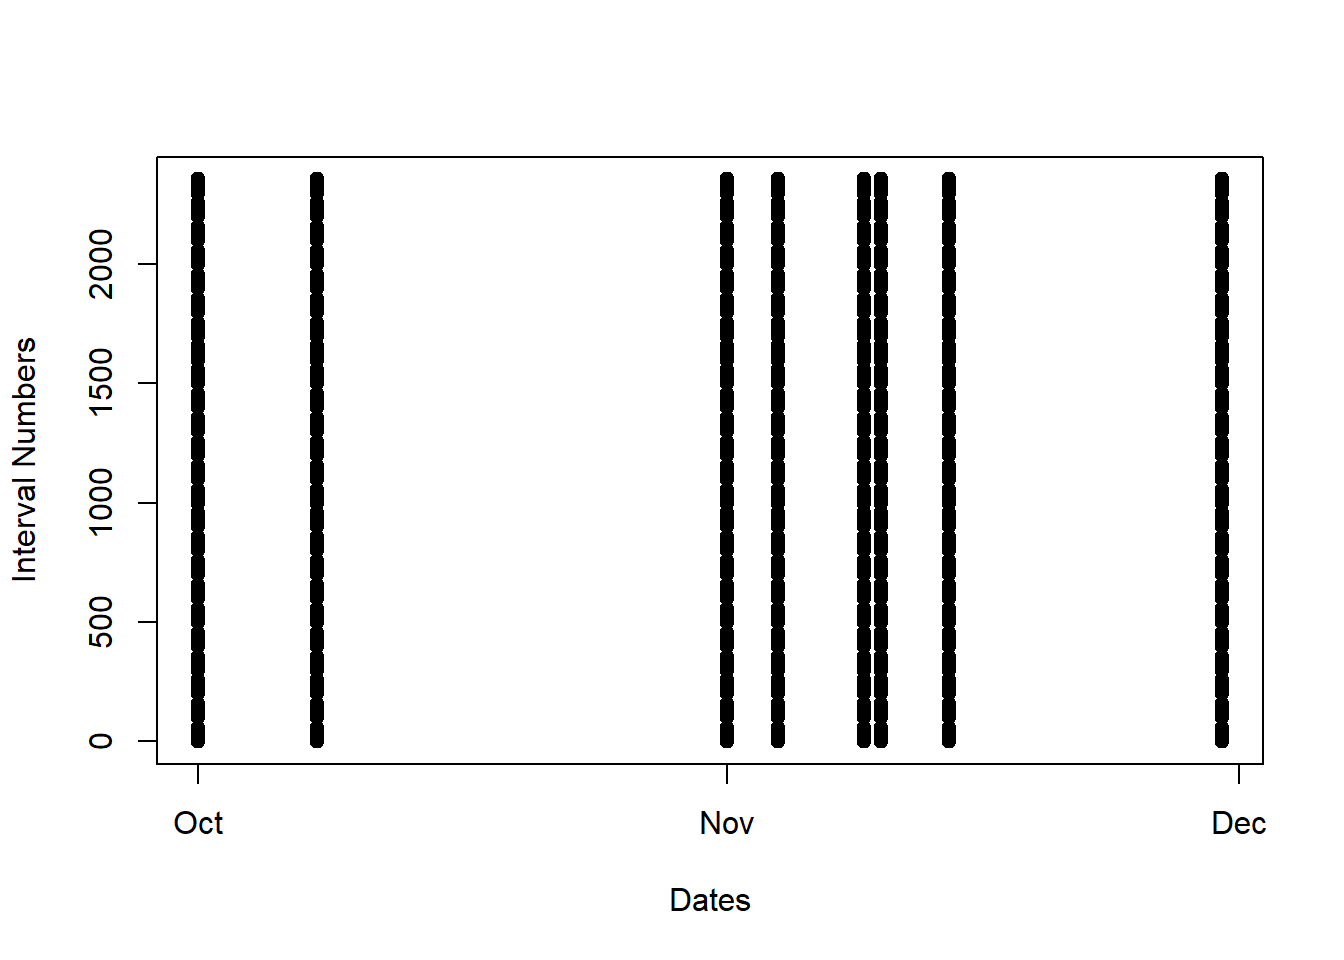
\includegraphics{Course_Project_1_for_Reproducible_Research_files/figure-latex/IDMIss-1.pdf}

Looks like the 2304 missing values are clustered on just a few days--but
across all intervals for those days. Therefore, the means for those
intervals should be good substitutions for the missing values. Now if I
can only figure out where I put those means . . . .

\begin{Shaded}
\begin{Highlighting}[]
\NormalTok{intMnSteps <-}\StringTok{ }\KeywordTok{with}\NormalTok{(df, }\KeywordTok{tapply}\NormalTok{(steps, df}\OperatorTok{$}\NormalTok{interval, mean, }\DataTypeTok{na.rm =} \OtherTok{TRUE}\NormalTok{)) ##Calculate the means}
\NormalTok{missings}\OperatorTok{$}\NormalTok{steps <-}\StringTok{ }\NormalTok{intMnSteps }\CommentTok{# Replace missing values}
\NormalTok{numMissingMissings <-}\StringTok{ }\KeywordTok{sum}\NormalTok{(}\KeywordTok{is.na}\NormalTok{(missings}\OperatorTok{$}\NormalTok{steps)) ## Check it. }
\end{Highlighting}
\end{Shaded}

Good enough. There are now 0 missing step values in what was a dataset
made up entirely of step values.

Now put the what-used-to-be-missing data into the data frame that we're
going to make next, which will be a dataset of all \emph{non}missing
step values in the original data set. My blood sugar must be getting low
because I can't believe I just wrote that. I'm not even sure it makes
sense.

\paragraph{8. Create a date set with imputed values instead of missing
values.}\label{create-a-date-set-with-imputed-values-instead-of-missing-values.}

\begin{Shaded}
\begin{Highlighting}[]
\NormalTok{df2 <-}\StringTok{ }\KeywordTok{na.omit}\NormalTok{(df) ## omit the missing values}
\NormalTok{numMissingdf2 <-}\StringTok{ }\KeywordTok{sum}\NormalTok{(}\KeywordTok{is.na}\NormalTok{(df2}\OperatorTok{$}\NormalTok{steps)) ## Check it}
\NormalTok{df2 <-}\StringTok{ }\KeywordTok{rbind}\NormalTok{(df2, missings)}
\NormalTok{df2 <-}\StringTok{ }\NormalTok{df2[}\KeywordTok{order}\NormalTok{(df2}\OperatorTok{$}\NormalTok{date), ]}
\NormalTok{totMissingAfterAllThat <-}\StringTok{ }\KeywordTok{sum}\NormalTok{(}\KeywordTok{is.na}\NormalTok{(df2}\OperatorTok{$}\NormalTok{steps))}
\end{Highlighting}
\end{Shaded}

After creating a dataset with 0 missing values in it, we put the two
data sets together and check for missing values. There are 0 of them.
Excellent.

\paragraph{9. Create a histogram of the total number of steps taken each
day after missing values are
imputed.}\label{create-a-histogram-of-the-total-number-of-steps-taken-each-day-after-missing-values-are-imputed.}

Recycle the default ``df'' dataframe name and reuse the code from above.

\begin{Shaded}
\begin{Highlighting}[]
\NormalTok{df <-}\StringTok{ }\NormalTok{df2}
\NormalTok{df}\OperatorTok{$}\NormalTok{date <-}\StringTok{ }\KeywordTok{strptime}\NormalTok{(df}\OperatorTok{$}\NormalTok{date, }\StringTok{"%Y-%m-%d"}\NormalTok{)}
\NormalTok{dates <-}\StringTok{ }\NormalTok{df}\OperatorTok{$}\NormalTok{date}
\NormalTok{uniqueDays <-}\StringTok{ }\KeywordTok{unique}\NormalTok{(df}\OperatorTok{$}\NormalTok{date)}
\NormalTok{uniqueInts <-}\StringTok{ }\KeywordTok{unique}\NormalTok{(df}\OperatorTok{$}\NormalTok{interval)}
\NormalTok{totUniqueDays <-}\StringTok{ }\KeywordTok{length}\NormalTok{(uniqueDays)}
\NormalTok{totUniqueInts <-}\StringTok{ }\KeywordTok{length}\NormalTok{(uniqueInts)}
\NormalTok{steps <-}\StringTok{ }\KeywordTok{split}\NormalTok{(df}\OperatorTok{$}\NormalTok{steps, dates}\OperatorTok{$}\NormalTok{yday)}
\NormalTok{totStepsDay <-}\StringTok{ }\KeywordTok{sapply}\NormalTok{(steps, sum, }\DataTypeTok{na.rm=}\OtherTok{TRUE}\NormalTok{)}
\KeywordTok{str}\NormalTok{(totStepsDay)}
\end{Highlighting}
\end{Shaded}

\begin{verbatim}
##  Named num [1:61] 10766 126 11352 12116 13294 ...
##  - attr(*, "names")= chr [1:61] "274" "275" "276" "277" ...
\end{verbatim}

\begin{Shaded}
\begin{Highlighting}[]
\KeywordTok{hist}\NormalTok{(totStepsDay, }\DataTypeTok{main =} \StringTok{"Total Steps per Day with Imputed Values for Missing"}\NormalTok{,}
     \DataTypeTok{xlab =} \StringTok{"Steps per Day"}\NormalTok{, }\DataTypeTok{ylab =} \StringTok{"Frequency"}\NormalTok{)}
\end{Highlighting}
\end{Shaded}

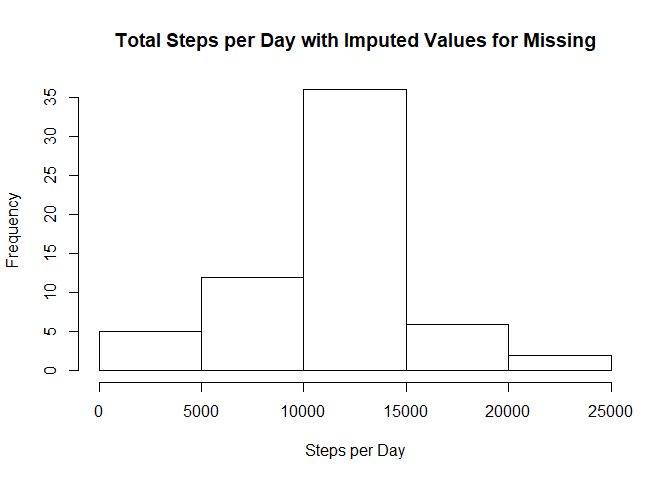
\includegraphics{Course_Project_1_for_Reproducible_Research_files/figure-latex/recycleReuse-1.pdf}

I like the shape of those data.

\begin{Shaded}
\begin{Highlighting}[]
\NormalTok{df2mnsteps <-}\StringTok{ }\KeywordTok{mean}\NormalTok{(totStepsDay, }\DataTypeTok{na.rm =} \OtherTok{TRUE}\NormalTok{)}
\NormalTok{df2mdsteps <-}\StringTok{ }\KeywordTok{median}\NormalTok{(totStepsDay, }\DataTypeTok{na.rm =} \OtherTok{TRUE}\NormalTok{)}
\NormalTok{meandiff <-}\StringTok{ }\NormalTok{df2mnsteps }\OperatorTok{-}\StringTok{ }\NormalTok{mnsteps}
\NormalTok{meddiff <-}\StringTok{ }\NormalTok{df2mnsteps }\OperatorTok{-}\StringTok{ }\NormalTok{mdsteps}
\end{Highlighting}
\end{Shaded}

\begin{itemize}
\tightlist
\item
  We \emph{used} to have a mean of 9354.23. Our new mean total steps is
  10766.19, a difference of 1411.96.\\
\item
  Median total steps \emph{was} 10395. Now it's 10766.19, the same as
  the mean. That's a difference of 371.19. The mean and the median are
  the same because we used the mean to replace missing the missing
  values. There are so many means with that exact value that the value
  became the median.\\
\item
  Most importantly, the data look a lot more parametric.
\end{itemize}

\paragraph{10. Panel plot comparing the average number of steps taken
per 5-minute interval across weekdays and
weekends}\label{panel-plot-comparing-the-average-number-of-steps-taken-per-5-minute-interval-across-weekdays-and-weekends}

First we mess around until the data are in the format we need for the
analysis. Create a new variable with day-of-the-week information it, set
it to 0 in all cases, then set it to 1 for weekdays. The remainder
should be weekends, but actually I'm not thrilled with that logic.

We know the data set has no missing steps because we imputed the men for
missing steps. So let's check for missing dates, just in case.

\begin{Shaded}
\begin{Highlighting}[]
\NormalTok{missdate <-}\StringTok{ }\KeywordTok{sum}\NormalTok{(}\KeywordTok{is.na}\NormalTok{(df}\OperatorTok{$}\NormalTok{date))}
\end{Highlighting}
\end{Shaded}

There are 0 of them.

Good. We can use sloppy logic, which follows.

\begin{Shaded}
\begin{Highlighting}[]
\NormalTok{dates <-}\StringTok{ }\NormalTok{df}\OperatorTok{$}\NormalTok{date}
\NormalTok{df}\OperatorTok{$}\NormalTok{wkdays <-}\StringTok{ }\NormalTok{dates}\OperatorTok{$}\NormalTok{wday }
\KeywordTok{summary}\NormalTok{(df}\OperatorTok{$}\NormalTok{wkdays)}
\end{Highlighting}
\end{Shaded}

\begin{verbatim}
##    Min. 1st Qu.  Median    Mean 3rd Qu.    Max. 
##       0       1       3       3       5       6
\end{verbatim}

\begin{Shaded}
\begin{Highlighting}[]
\NormalTok{df}\OperatorTok{$}\NormalTok{isWeekend <-}\StringTok{ }\KeywordTok{is.weekend}\NormalTok{(df}\OperatorTok{$}\NormalTok{wkdays)}
\KeywordTok{summary}\NormalTok{(df}\OperatorTok{$}\NormalTok{isWeekend)}
\end{Highlighting}
\end{Shaded}

\begin{verbatim}
##    Mode   FALSE    TRUE 
## logical   12384    5184
\end{verbatim}

\begin{Shaded}
\begin{Highlighting}[]
\NormalTok{weekendDays <-}\StringTok{ }\KeywordTok{sum}\NormalTok{(df}\OperatorTok{$}\NormalTok{isWeekend)}
\NormalTok{weekDays <-}\StringTok{ }\KeywordTok{length}\NormalTok{(dates) }\OperatorTok{-}\StringTok{ }\NormalTok{weekendDays}
\end{Highlighting}
\end{Shaded}

So we have 12384 weekdays and 5184 weekend days. Sounds reasonable
enough.

Make the weekday - weekend factor variable.

\begin{Shaded}
\begin{Highlighting}[]
\NormalTok{df}\OperatorTok{$}\NormalTok{dayType <-}\StringTok{ }\KeywordTok{ifelse}\NormalTok{(df}\OperatorTok{$}\NormalTok{isWeekend }\OperatorTok{==}\StringTok{ "FALSE"}\NormalTok{, df}\OperatorTok{$}\NormalTok{dayType <-}\StringTok{ "Weekday"}\NormalTok{, df}\OperatorTok{$}\NormalTok{dayType <-}\StringTok{ "Weekend Day"}\NormalTok{)}
\NormalTok{df}\OperatorTok{$}\NormalTok{dayType <-}\StringTok{ }\KeywordTok{as.factor}\NormalTok{(df}\OperatorTok{$}\NormalTok{dayType)}
\KeywordTok{summary}\NormalTok{(df}\OperatorTok{$}\NormalTok{dayType)}
\end{Highlighting}
\end{Shaded}

\begin{verbatim}
##     Weekday Weekend Day 
##       12384        5184
\end{verbatim}

\begin{Shaded}
\begin{Highlighting}[]
\NormalTok{stepsPerDay <-}\StringTok{ }\KeywordTok{aggregate}\NormalTok{(steps }\OperatorTok{~}\StringTok{ }\NormalTok{interval }\OperatorTok{+}\StringTok{ }\NormalTok{dayType, }\DataTypeTok{data =}\NormalTok{ df, mean)}
\KeywordTok{names}\NormalTok{(stepsPerDay) <-}\StringTok{ }\KeywordTok{c}\NormalTok{(}\StringTok{"interval"}\NormalTok{, }\StringTok{"dayType"}\NormalTok{, }\StringTok{"steps"}\NormalTok{)}
\end{Highlighting}
\end{Shaded}

\begin{Shaded}
\begin{Highlighting}[]
\KeywordTok{xyplot}\NormalTok{(steps }\OperatorTok{~}\StringTok{ }\NormalTok{interval }\OperatorTok{|}\StringTok{ }\NormalTok{dayType, stepsPerDay, }\DataTypeTok{type =} \StringTok{"l"}\NormalTok{, }\DataTypeTok{layout =} \KeywordTok{c}\NormalTok{(}\DecValTok{1}\NormalTok{, }\DecValTok{2}\NormalTok{), }
    \DataTypeTok{xlab =} \StringTok{"Interval"}\NormalTok{, }\DataTypeTok{ylab =} \StringTok{"Number of Steps"}\NormalTok{)}
\end{Highlighting}
\end{Shaded}

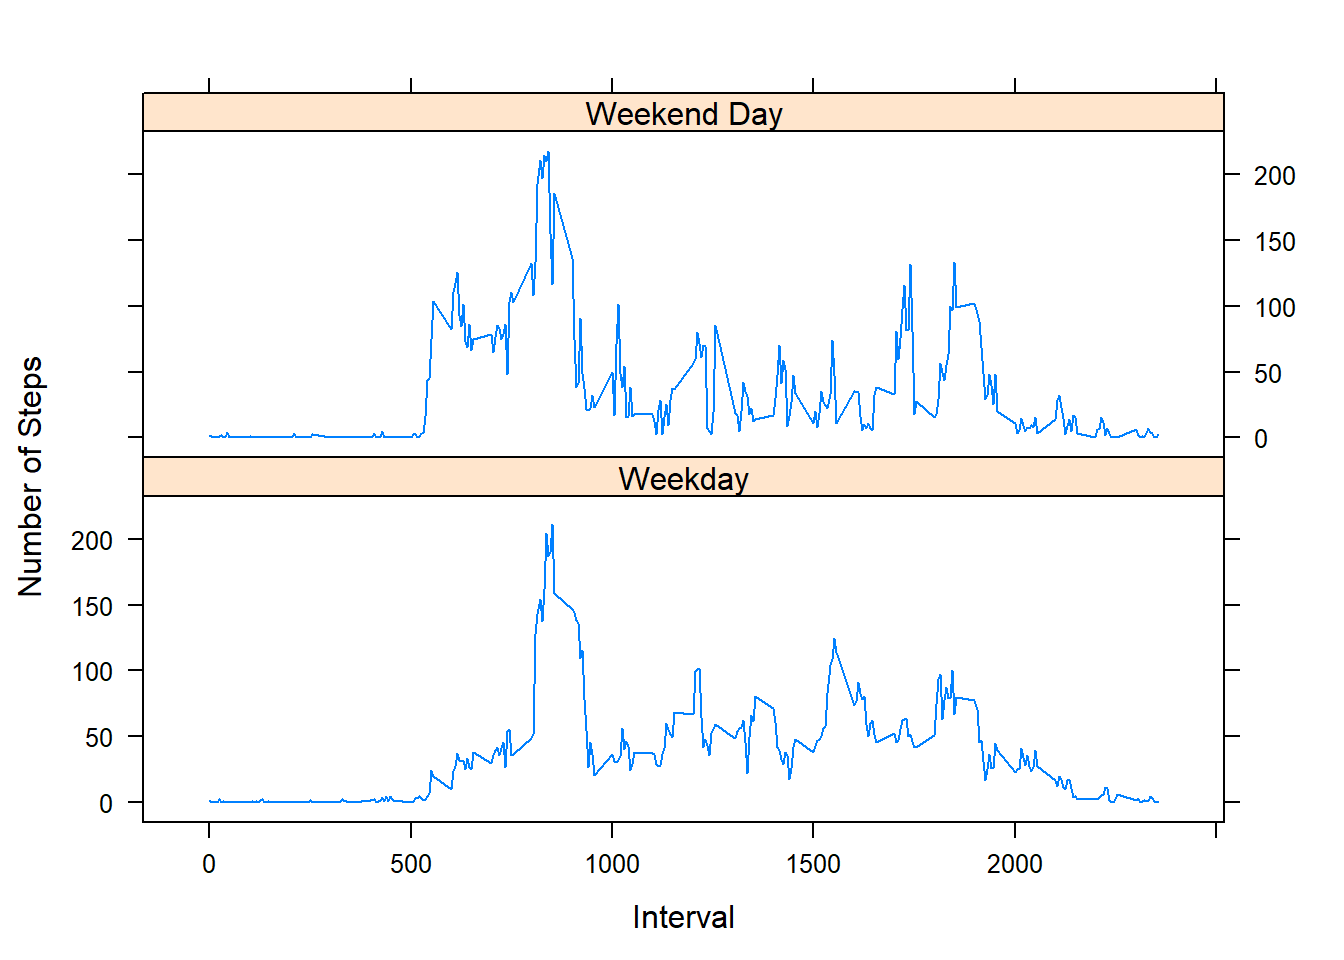
\includegraphics{Course_Project_1_for_Reproducible_Research_files/figure-latex/makeFacetedTimeSeriesPlot-1.pdf}

Commit your completed
\color{red}{\verb|PA1_template.Rmd|}PA1\_template.Rmd file to the
\color{red}{\verb|master|}master branch of your git repository (you
should already be on the \color{red}{\verb|master|}master branch unless
you created new ones) Commit your PA1\_template.md and
PA1\_template.html files produced by processing your R markdown file
with knit2html() function in R (from the knitr package) by running the
function from the console. If your document has figures included (it
should) then they should have been placed in the figure/ directory by
default (unless you overrided the default). Add and commit the figure/
directory to your git repository so that the figures appear in the
markdown file when it displays on github. Push your
\color{red}{\verb|master|}master branch to GitHub. Submit the URL to
your GitHub repository for this assignment on the course web site. In
addition to submitting the URL for your GitHub repository, you will need
to submit the 40 character SHA-1 hash (as string of numbers from 0-9 and
letters from a-f) that identifies the repository commit that contains
the version of the files you want to submit. You can do this in GitHub
by doing the following

Going to your GitHub repository web page for this assignment Click on
the ``?? commits'' link where ?? is the number of commits you have in
the repository. For example, if you made a total of 10 commits to this
repository, the link should say ``10 commits''. You will see a list of
commits that you have made to this repository. The most recent commit is
at the very top. If this represents the version of the files you want to
submit, then just click the ``copy to clipboard'' button on the right
hand side that should appear when you hover over the SHA-1 hash. Paste
this SHA-1 hash into the course web site when you submit your
assignment. If you don't want to use the most recent commit, then go
down and find the commit you want and copy the SHA-1 hash.

\subsubsection{Project Requirements}\label{project-requirements}

\begin{itemize}
\tightlist
\item
  Valid GitHub URL
\item
  At least one commit beyond the original fork
\item
  Valid SHA-1
\item
  SHA-1 corresponds to a specific commit
\item
  Commit containing full submission
\end{itemize}


\end{document}
